\begin{tikzpicture}[x=0.116mm,y=-0.116mm]
  \node[anchor=north west,inner sep=0] at (0,0) {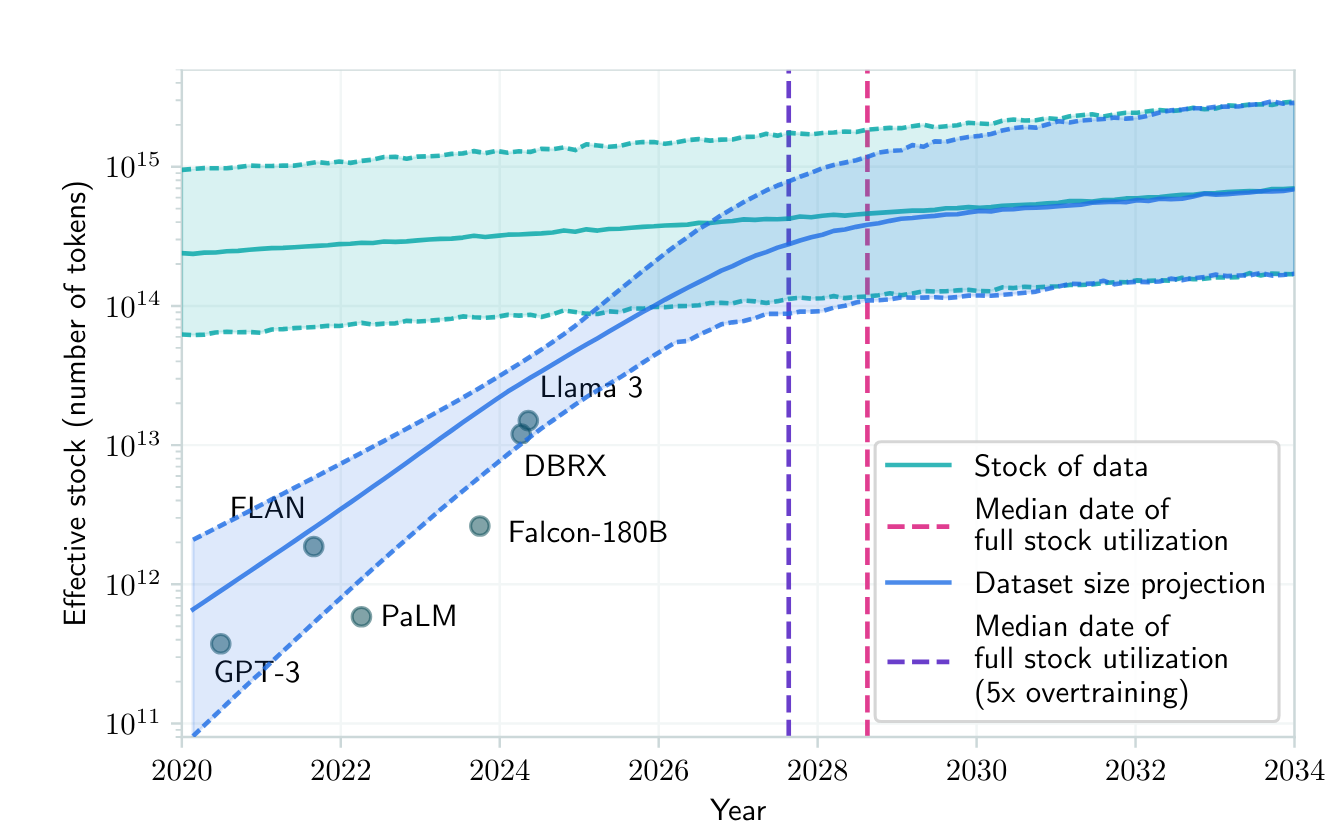
\includegraphics[width=154.976mm]{part6/visuals/data_stock.png}};
  \fill[white] (39,171) rectangle (100,682);
  \node[rotate=90,font=\small,fill=white,inner sep=2pt] at (70,425) {有效存量（词元数）};
  \fill[white] (680,789) rectangle (795,837);
  \node[font=\small] at (739,810) {年份};
  \fill[white] (965,449) rectangle (1269,715);
  \node[anchor=west,font={\fontsize{9}{10.5}\linespread{1}\selectfont}] at (970,467) {数据存量};
  \fill[white] (964,489) rectangle (1270,559);
  \node[anchor=west,align=left,font={\fontsize{9}{10.5}\linespread{1}\selectfont}] at (970,522) {全量数据用尽的\\中位年份};
  \fill[white] (964,565) rectangle (1270,604);
  \node[anchor=west,font={\fontsize{9}{10.5}\linespread{1}\selectfont}] at (970,582) {数据集规模预测};
  \fill[white] (964,607) rectangle (1270,710);
  \node[anchor=west,align=left,font={\fontsize{9}{10.5}\linespread{1}\selectfont}] at (970,657) {全量数据用尽的\\中位年份\\（5 倍超额训练）};
\end{tikzpicture}
